\newpage

\section{Vizuálna pozornosť}
\label{saliency}
	
Termín vizuálna pozornosť možno definovať ako súbor všetkých faktorov, ktoré ovplyvňujú naše mechanizmy výberu podstatných častí v scéne a jej spracovanie, nezáležiac od toho, aké tieto mechanizmy sú (či už riadené stimulmi, očakávaniami, pamaťou, atď.) \cite{borji2013state}.

Tento pojem je často zamieňaný s vizuálnou výraznosťou, avšak tieto dva termíny nevyjadrujú úplne to isté. Presnejšou definíciou vizuálnej výraznosti (z angl. visual saliency) je, že sa jedná o značne subjektívnu perceptuálnu vlastnosť, vďaka ktorej niektoré veci vo svete (v scéne) vyčnievajú v porovnaní so svojimi susedmi kvôli ich vlastnostiam ako farba, jas, kontrast či orientácia \cite{itti2007visual}. Upútanie pozornosti ovplyvňujú mechanizmy spracovania scény, ktoré možno rozdeliť na dve skupiny:
\begin{itemize}
	\item spracovanie „zdola nahor“ (z angl. bottom-up) %- riadená čisto iba pútavými stimulmi, ktoré sú v podstate známkou toho, že „táto lokácia je značne odlišná od svojho okolia a stojí za pozornosť.“\ Je rýchla a nevedomá.
	\item spracovanie „zhora nadol“ (z angl. top-down) %- riadená tzv. predvídateľnými mechanizmami, ako napríklad hľadaním niečoho konkrétneho na webovej stránke. Je pomalšia, vedomá a ovplyvnená našou pamaťou. 
	
\end{itemize}


\subsection{Spracovanie zdola nahor}
Vizuálne stimuly, ktoré upútajú pozornosť automaticky, mimovoľne, sa nazývajú bottom-up stimuly (alebo kontextovo riadené). Práve tieto riadia našu pozornosť a v podstate sú akousi známkou (ukazovateľom), že táto lokácia (alebo objekt v nej) je značne odlišná od svojho okolia a presne preto stojí za pozornosť. Ich príkladom môžu byť značky pri pozemných komunikáciách, bezpečnostné prvky vo vozidlách, ale aj správne umiestnené titulky v novinách, blogoch, či dizajnérmi nesprávne umiestnená reklama na webových stránkach zbytočne odtrhujúca našu pozornosť od podstatných vecí. 

Hlavnou charakteristikou tohto spracovania je nevedomosť (obvykle bez predošlých informácií o pozorovanej scéne) a rýchlosť - priemerné spracovanie jedného objektu v scéne je na úrovni od 20 do 50 milisekúnd\cite{itti2001computational}.


\subsection{Zhora nadol spracovanie}
Tento typ spracovania vizuálnych signálov sa oproti vyššie uvedenému líši viacerými vecami. Tou prvou je, že sa riadi tzv. predvídateľnými mechanizmami a prináša so sebou bližšie nešpecifikovanú vedomosť o pozorovanej scéne - pozorovateľ má isté informácie ako napríklad predošlé skúsenosti, spomienky, alebo hľadá v scéne nejaký konkrétny objekt. Z tohto dôvodu sa nazýva aj spracovaním založeným na vedomostiach (z angl. knowledge-based processing\cite{goldstein2008blackwell}) alebo údajoch (z angl. data-driven processing\cite{gregory1974concepts})

Druhým veľkým rozdielom oproti spracovaniu zdola nahor je jeho rýchlosť, priemerný čas spracovania vizuálneho signálu sa pohybuje na úrovni 200 milisekúnd\cite{itti2001computational} a viac, čo je výrazne pomalšie.

% TODO dake shity dopisat este


\newpage

\section{Neurónové siete}
\label{nn}

Neurónová sieť - pojem reprezentujúci značne abstraktný výpočtový model, ktorého princíp fungovania bol postavený na reálnych biologický neurosystémoch. Ako už zo základnej školy vieme, základnou stavebnou jednotkou živých organizmov je bunka. Jej špecializovaným derivátom je nervová bunka - neurón, stavebný kameň nervových systém. Pri neurónových sieťach je základnou jednotkou rovnako neurón (avšak nie živý ale umelý), respektíve jeho matematické vyjadrenie. To predpokladá, že umelý neurón je schopný spracovať \textit{N} vstupov a k nim poskytnúť \textit{M} výstupov. Jedna zo starších matematický špecifikácii ho popisuje nasledovne:

	\begin{equation}
		o_i ^{k+1} = f\left ( \sum_{j+1}^{N} w_{ij}^{k} * o_j^k - \theta_i^{k+1}  \right )
	\end{equation}
	
Pre vyššie uvedené platí: 
\newline
\textit{0 \textless i ≤ M
\newline
0 \textless j ≤ N}
\newline
\(o_i^{k+1}\)  - výstupná hodnota i-teho neurónu patriaceho k+1 vrstve 
\newline
\textit{k} - číslo vrstvy
\newline
\(\theta_{ij}^{k}\) - prah stimulácie i-teho neurónu k+1 vrstvy
\newline
\(w_{ij}^{k}\) - váha medzi i-tym neurónom vrstvy k+1 a j-tym neurónom vrstvy k 
\newline 
\textit{f()} - aktivačná funkcia
\newline
	
Modernejšie prístupy však odstránili prah stimulácie neurónu a miesto neho pridali tzv. predsudok (z angl. bias), ktorý reprezentuje predpokladanú (s časom sa meniacu) hodnotu stimulácie neurónu na ďalšej vrstve. Pre vysvetlenie hypoteticky predpokladajme, že máme umelý neurón a chceme, aby spracoval \textit{m+1} vstupov so signálmi od \(x_0\) po \(x_m\) a váhami od \(w_0\) po \(w_m\). Pre \(x_0\) pridelíme hodnotu +1, vďaka čomu sa stane predsudkom (biasom) k vstupu s \(w_{k0} = b_k\). Týmto postupom nám teda zostane iba \textit{m} vstupov so signálmi od \(x_1\) po \(x_m\). Popisovaný postup ako aj výstup z k-teho neurónu matematicky vyjadruje rovnica \ref{eq:new_neuron} nižšie:

	\begin{equation}
		\label{eq:new_neuron}
		y_k = \phi (\sum_{j=0}^{m} w_{kj}*x_j)
	\end{equation}
	
Pre vyššie uvedené platí:
\newline
\(y_k\) - výstup k-teho neurónu
\newline
\(w_{kj}\) - váha j-teho neurónu spojeného s k-tym neurónom na ďalšej vrstve
\newline
\(x_j\) - j-ty neurón 
\newline
\(\phi\) - aktivačná funkcia
\newline

Takéto umelé neuróny sú potom umiestnené na vrstvách s prepojeniami napr. do ďalších vrstiev. Štandardne sa prvá vrstva nazýva vstupná a posledná výstupná. Tie medzi sebou ďalej môžu mať niekoľko ďalších vrstiev rôzneho typu. Tieto vrstvy sa nazývajú skrytými a obvykle práve tieto bývajú kľúčové pri učení sa a predikciách. Neuróny každej vrstvy navyše môžu obsahovať aj aktivačnú funkciu (klasicky býva pre všetky neuróny na vrstve rovnaká), ktorá definuje (upravuje) výstup z neurónu pre vstup alebo sériu vstupov.
	
\subsection{Aktivačné funkcie}\label{activation_functions}

Aktivačná funkcia predstavuje matematické vyjadrenie použité k aproximácii vplyvu na neurón, zjednodušene by bolo možné povedať, že pre sériu vstupov definuje výstupy. Aktivačných funkcií existuje niekoľko typov, každá vhodná na iný typ úloh. Ako príklad je možné uviesť nasledujúce: 
	\begin{itemize}
		\item {\textbf{Softmax}}
		
		Funkcia softmax\footnote{http://eli.thegreenplace.net/2016/the-softmax-function-and-its-derivative/} (inak aj normalizovaná exponenciálna funkcia) normalizuje daný  \textit{n} dimenzionálny vektor tak, že upraví jeho hodnoty do rozsahu (0,1), pričom ich súčet bude rovný 1. Jej matimatické vyjadrenie je nižšie. 
		\begin{equation}
		S_{vec_j} = \frac{e^{vec_j}}{\sum_{i=1}^{n}e^{vec_i}}
		\end{equation}
		
		Pre vyššie uvedené vyjadrenie platí:
		
		\(\forall{\ j\ }\in\ 1..n\)
		
		\(vec \) - konkrétny vector
		
		Keď si ako príklad vezmeme jednoduchý vektor [1, 2, 3], výsledok po aplikovaní softmaxu bude [0.09, 0.24, 0.67]. Ako môžeme vidieť, funkcia sa väčšinou používa na zvýraznenie väčších hodnôt a zárove\ potlačenie hodnôt, ktoré sú výrazne menšie ako maximálna hodnota. 
		
		\item {\textbf{ReLU}}
		
		Upravená lineárna jednotka (z angl. rectified linear unit) je funkcia 
		v tvare:
		\begin{equation}
		f(x) = max (0, x)
		\end{equation}
		kde \textit{x} je vstup do neurónu. Používa sa vďaka svojej jednoduchosti, keďže neobsahuje žiadne komplikované výpočty, čoho dôsledkom je aj jej značná rýchlosť. Jej využitie je možné pozorovať napríklad pri hlbokých neurónových sieťach.
		
		\item{\textbf{Softplus}}
		
		Je v podstate aproximáciou k predošlej ReLU s matematickým vyjadrením:
		\begin{equation}
		f(x)=ln (1 + e^x)
		\end{equation}
		Rovnako ako pri ReLU je oborom hodnôt interval (0, \(\infty\)). Jej využitie je napríklad pri rozoznávaní reči.
		
		\item{\textbf{Sigmoid}}
		
		Táto funkcia sa používa hlavne keď je potrebné pracovať s pravdepodobnosťami, keďže jej výstup tvorí interval (0, 1). Jej matematické vyjadrenie je nasledovné:
		\begin{equation}
		S(t) = \frac{t}{1-e^{-t}}
		\end{equation}
		
		\item {\textbf{Tanh}}
		
		Hyberbolický tangens. Často sa používa v rovnakých prípadoch ako Sigmoid, keďže matematicky sa dá vyjadriť aj za použitia Sigmoidu. Jeho vzorec je nasledovný:
		\begin{equation}
			tanh(x)=\frac{cosh(x)}{sinh(x)}=Sigmoid(2x)-Sigmoid(-2x)=\frac{e^{2x}-1}{e^{2x}+1}
		\end{equation}
	\end{itemize}
	
\subsection{Učenie sa neurónovej siete}
	
Základným prvkom toho, aby bola neurónová sieť schopná riešiť úlohy je učenie sa. Existujú viaceré typy učenia sa neurónovej siete, základnými sú učenie sa s učiteľom (z angl. supervised learning), učenie sa bez učiteľa (z angl. unsupervised learning\cite{unsupervised}) a učenie sa posilňovaním (z angl. reinforcement leatning\cite{mnih2013playing}). 

\subsubsection{Učenie sa s učiteľom}
Učenie s učiteľom prebieha na predpripravenom datasete, ktorý musí obsahovať nejaké testovacie vstupné dáta (pre ktoré chceme vypočítať výstupnú funkciu) a takzvané štítky (z angl. labels), ktoré sú v podstate naše očakaváne výstupy. Najčastejším príkladom tohto typu učenia je algoritmus spätného šírenia chyby (z angl. backpropagation\cite{nielsen2015neural}).

\paragraph{Algoritmus spätného šírenia chyby}
Hlavným princípom je snaha o minimalizovanie chyby predikcie pri učení a to tak, že po predikcii pri učení sa vypočíta hodnota chyby na poslednej výstupnej vrstve voči očakávanému výstupu (spomínaným štítkom). Tá sa potom tzv. "šíri" \ späť k vstupnej vrstve a vzhľadom na jej hodnotu sa postupne aktualizujú váhy jednotlivých neurónov.

Príklad použitia tohto algoritmu možno nájsť v jednoduchej neurónovej sieti určenej k riešeniu problému funkcie XOR\cite{neuron}. Vstupné dáta je nutné reprezentovať ako dvojicu jednotiek a núl. Pre vstupnú dvojicu napríklad \textit{[0,1]} je očakávaným výstupom číslo \textit{1}, pre hodnotu \textit{[0,0]} je to \textit{0}. Tieto očakávané hodnoty zároveň označíme za spomínané štítky. Takto pripravíme celý dataset pre trénovanie, mal by byť dostatočne rozsiahly aby sa dosiahla maximálna presnosť (odhadnúť aké množstvo dát už možno považovať za dostatočné je značne netriviálny problém). Sieti sú potom počas učenia predkladané vstupy a štítky, na základe vypočítanej chyby sú potom predikcie upravované až kým chyba nie je úplne minimalizovaná. Spomínaný problém veľkosti dostatočne rozsiahleho datasetu je považovaný za jeden z hlavných mínusov učenia s učiteľom.

	
\paragraph{Učenie sa viacerých inštancií}

MIL\cite{minhas2012multiple} - skratka pre anglický výraz Multiple Instance Learning, čiže učenie sa viacerých inštancií, je variácia učenia s učiteľom. Miesto obdržania individuálne oštítkovaných inštancií (reprezentujú triedy, ktoré chceme predikovať),  obdrží model set oštítkovaných vreciek (z angl. bags), z ktorého každé obsahuje niekoľko inštancií. V prípade jednoduchej binárnej klasifikácie je celé vrecko označené ako negatívna vzorka, ak všetky inštancie vo vnútri sú negatívne. Pokiaľ ale obsahuje aspoň jednu pozitívnu, je označené ako pozitívna vzorka. Pri zložitejších triedach si ako príklad môžeme uviesť predikciu nejakej cieľovej triedy pre obrázok na základe vizuálneho obsahu. Cieľová trieda bude \textit{"pláž"} pre obrázok, ktorý obsahuje  \textit{"piesok"} a \textit{"vodu"}. V terminológii MIL je teda obrázok popísaný ako vrecko, matematicky reprezentované nasledovne:
	\begin{equation}
		X = \{X_1, ..., X_N\}
	\end{equation}

$X_{i}$ reprezentuje vektor čŕt (inštanciu) extrahové z prislúchajúceho i-teho regiónu obrázku a \textit{N} je celkový počet regiónov (inštancií) v obrázku. Vrecko je označené pozitívne  (\textit{"pláž"})  v prípade, že obsahuje oba regióny (inštancie) \textit{"piesok"} a \textit{"voda"}.

\subsubsection{Učenie sa bez učiteľa}
Základný popis o učení bez učiteľa hovorí, že sa jedná o odvodenie funkcie k popisu skrytej vnútornej štruktúry z neoštítkovaných dát. Dalo by sa teda tvrdiť, že tu nie sú žiadne signály, chyba či ukazovatele, ktoré by nám napovedali alebo ohodnocovali to, ako dobré je potenciálne riešenie (predikcia). Tento typ učenia je široko používaným napr. v oblasti dátových analýz.

\subsubsection{Učenie posilňovaním}
Tento typ učenia má podobne ako učenie s učiteľom k dispozícii istú spätnú väzbu o kvalite predikcií počas trénovania, nie je to však tak konkrétna informácia ako chyba predikcie voči správnym výstupom. Spätná väzba predstavuje ohodnotenie predikcie buď odmenou alebo trestom, v závislosti od toho aká dobrá bola. Hlavným cieľom je, ako by sa dalo očakávať, maximalizovanie získanej odmeny. Tú neurónová sieť získava metódou pokus- omyl pri upravovaní váh počas trénovania. Tento postup do značnej miery simuluje učenie sa v reálnom svete. Najčastejšie sa používa pri algoritmoch, ktoré sú stavané na hranie doskových alebo počítačových hier. 


\subsubsection{Optimizačné algoritmy}
\label{optimizers}
V kombinácii s algoritmami učenia sa používajú optimizačné algoritmy, ktorých cieľom je nájdenie minima funkcie medzi váhami. Medzi základné optimizéry patria:

\begin{itemize}
	\item \textbf{Gradient descent optimizer \cite{gradient_descent}:}
	
	Je to iteratívny algoritmus používaný k nájdeniu lokálneho minima funkcie, kedy podniká kroky k nájdeniu záporného gradientu\footnote{ zmena veličiny v závislosti od inej premennej} funkcie v aktuálnom bode. To je využívané pri určovaní rýchlosti učenia sa neurónovej siete. Existujú 3 hlavné varianty gradient descent optimizéru, ktoré počítajú sklon (gradient) funkcie. Delia sa hlavne podľa množstva dát určenému k spracovaniu, kedy sa robí kompromis medzi presnosťou aktualizácie parametra a časom, ktorý je potrebný na vykonanie tejto aktualizácie. Týmito typmi sú:
	\begin{itemize}
		\item{Dávkový gradient descent:}
		
		Z angl. Batch gradient descent. Gradient sa počíta pre celý tréningový dataset, takže pre jednu aktualizáciu je potrebné ho prejsť celý a preto môže byť veľmi pomalý. 
		\item {Stochaistický gradient descent:}
		
		Tento typ je presným kontrastom voči dávkovému gradient descentu. Aktualizácia sa uskutočňuje pre každú vzorku z tréningového datasetu. 
		\item{Mini-dávkový gradient descent:}
		
		Je kompromisom medzi predošlými dvomi typmi. Aktualizácia prebieha pre malú dávku (batch) z datasetu o veľkosti \textit{n} vzoriek.
	\end{itemize} 
	\item \textbf{Adam optimizer \cite{adam}:}
	
	V podstate vychádza priamo zo Stochaistického gradient descent optimizéru, resp. jeho modifikácie RMSProp algoritmu\cite{rms}. Rozdiel oproti Gradient descent optimizéru je ale v tom, že je schopný variabilne určovať rýchlosť učenia neurónovej siete.
	
	\item \textbf{Adadelta optimizer \cite{adadelta}:}
	
	Jedná sa o rozšírenie Adagrad optimizéru\cite{adagrad}, ktoré sa snaží zredukovať jeho agresívnu, monotónne klesajúcu rýchlosť učenia. Je robustnejší, prispôsobovanie spomínanej rýchlosti učenia je založené na pohyblivom okne aktualizácií gradientu namiesto akumulácie všetkých minulých gradientov, ako je to pri Adagrad optimizéri. Vďaka tomu je Adadelta schopný pokračovať v učení aj po veľkom množstve epoch a aktualizácií gradientu.\footnote{https://keras.io/optimizers/} 
	
	\item \textbf{Ftrl optimizer:}
	
	Vychádza z algoritmu učenia FTRL-Proximal\cite{ftrl}, celým názvom Nasleduj regularizovaného vodcu (z angl. Follow The (Proximal) Regularized Leader). Tento algoritmus je bez regularizácie v podstate identický s gradient descentom, avšak používa alternatívnu reprezentáciu koeficientov váh a tak môže byť regularizácia implementovaná efektívnejšie.
\end{itemize}

Aj keď neurónové siete dokážu efektívne riešiť veľké množstvo úloh, problémom stále zostáva mať k dispozícii dostatok dát k učeniu neurónovej siete ešte pred riešením úloh. Taktiež je potrebné mať dostatok výpočtovej sily, aby sa problém neriešil pridlhý čas, a dostatok pamäte, keďže neurónové siete jej potrebujú značné množstvo. 	
	 
	
\subsection{Typy neurónových sietí}

Neurónové siete majú niekoľko typov, ktoré  sa rozlišujú hlavne podľa spôsobu prepojenia neurónov, ale aj podľa typu úloh, na ktoré sú určené, či podľa počtu vrstiev neurónov alebo štýlu učenia. %doplnit zdroj
	
	
Najjednoduchší typ možno zobraziť ako jednu vstupnú vrstvu, jednu skrytú a jednu výstupnú, neuróny sú tu poprepájané z n-tej vrstvy do n+1 vrstvy, ako je možné vidieť na obrázku \ref{simple_nn}. Tento typ sa nazýva dopredná neurónová sieť (z angl. feedforward neural network) a môže mať aj viac ako len jednu skrytú vrstvu. Používa sa hlavne ak sa jedná  o predikciu nelineárnej funkcie (napríklad carbon-13 NMR chemické posuny alkánov\cite{feedforward}). 
	\begin{figure}[H]
		\begin{center}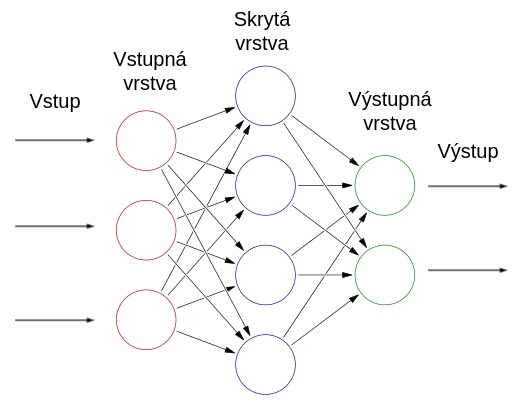
\includegraphics[scale=0.45]{simple_nn.jpg}\end{center}
		\caption[Jednoduchá neurónová sieť]{Príklad jednoduchej neurónovej siete}\label{simple_nn}
	\end{figure}

\subsubsection{Rekurentné neurónové siete}
Zložitejším typom  neurónových sietí sú rekurentné neurónové siete. Už z názvu vyplýva, že jednou z vecí, ktoré umožňujú, je rekurenciu. Vďaka nej prepojenia neurónov už nie sú jednosmerné len z jednej vrstvy na druhú, ale umožňuje prepojiť neuróny akokoľvek a tak vytvárať napríklad slučky či cykly (ukážka na obrázku \ref{rnn_image}).

\begin{figure}[H]
	\begin{center}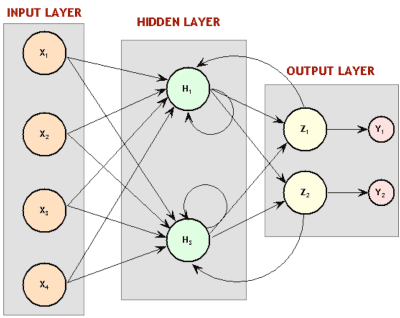
\includegraphics[scale=0.7]{rnn_model.png}\end{center}
	\caption[Jednoduchá rekurentná neurónová sieť]{Príklad jednoduchej rekurentnej neurónovej siete\label{rnn_image}\footnotemark}
	
\end{figure}
\footnotetext{http://www.mattmoocar.me/blog/RNNCountryLyrics/}

Vyššie uvedená funcionalita dovoľuje zachytiť aj dynamické časovo obmedzené správanie a používať kontext z minulosti, teda použiť niečo ako „pamäť“. Rekurentné siete majú veľké množstvo typov, od jednoduchších LSTM až po zložitejšie obojsmerné (z angl. bi-directional).

\paragraph{LSTM} 
LSTM\cite{gers1999learning} - skratka pre anglické pomenovanie Long short-term memory, čo v preklade znamená dlhá krátkodobá pamäť. Tento typ rekurentných sietí sa ukázal extrémne efektívny pri úlohách, kde je nutné pamätať si určitú informáciu (kratšieho charakteru) dlhý čas. Za to môžeme vďačiť LSTM jednotke, ktorej štandardná architektúra je zobrazená na obrázku \ref{lstm_unit_image}.

\begin{figure}[H]
	\begin{center}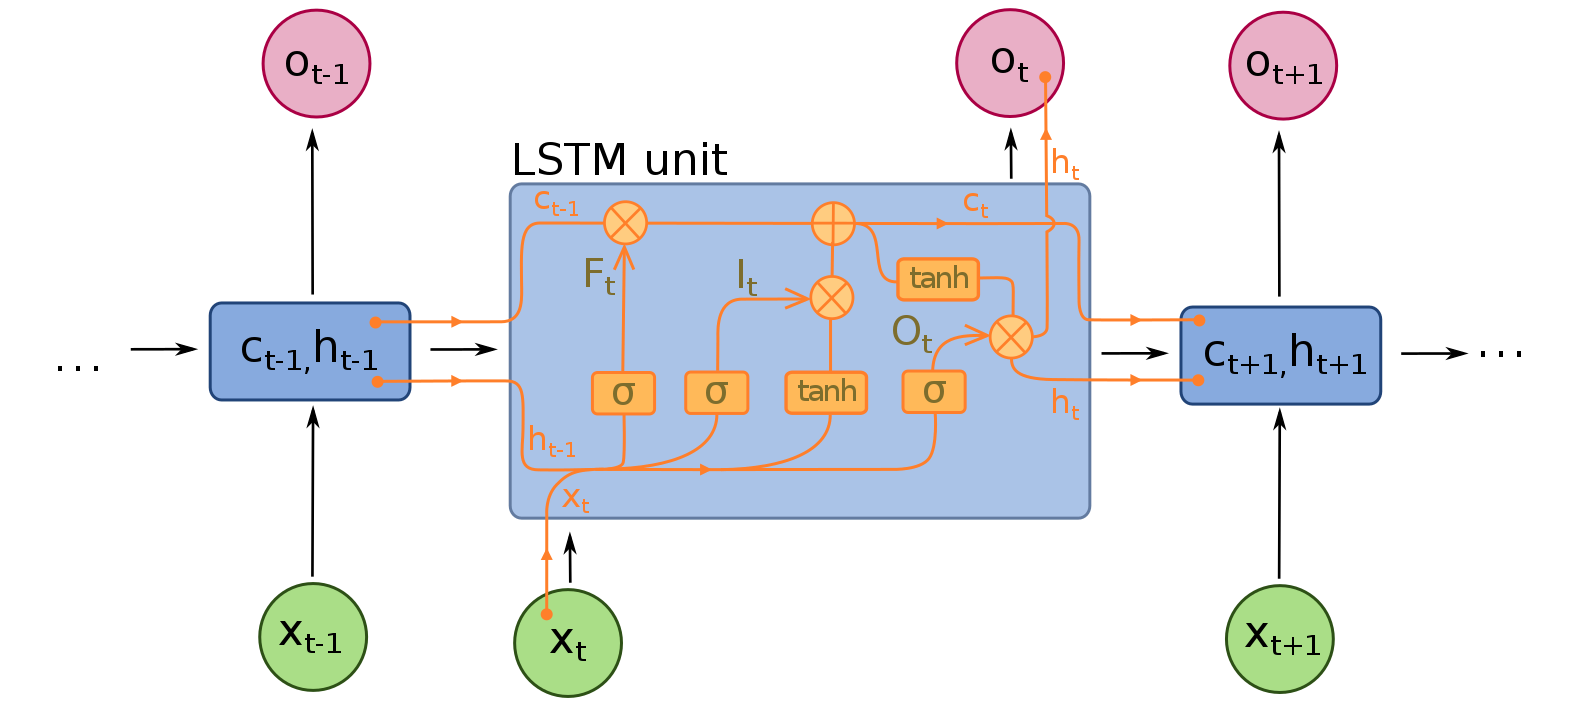
\includegraphics[scale=0.25]{lstm_unit.png}\end{center}
	\caption[Zobrazenie LSTM jednotky]{Ukážka štruktúry LSTM jednotky\label{lstm_unit_image}\footnotemark}
	
\end{figure}
\footnotetext{http://colah.github.io/posts/2015-08-Understanding-LSTMs/}

Na rozdiel od klasickejších rekurentných sietí, kde jednotka obsahuje jednu vrstvu neurónov, LSTM jednotka (bunka) obsahuje až štyri, každá špecializovaná na niečo iné. Na obrázku vyššie reprezentuje prvá horizontálna čiara v jednotke jej stav. Informácia tadiaľto prakticky len "tečie", s malými lineárnymi zmenami ako pridanie alebo odobratie. Tieto akcie sú opatrne regulované tzv. bránami.

Spodná horizontálna čiara reprezentuje postupné vstupy do štyroch vrstviev zobrazených na obrázku ako štvorce s aktivačnými funkciami ($\sigma$ - sigmoid, tanh). Vrstvy so sigmoid-om fungujú ako tzv. "strážcovia", vzhľadom na ich výstup v intervale \ <0,1> \ určujú aké veľké množstvo informácie má byť pustené ďalej (0 - nič, 1 - všetko). Týmto prakticky kontrolujú a udržujú stav celej bunky. Prvá sigmoid vrstva sa nazýva "zabúdacia brána" (z angl. forget gate layer) a určuje, aké množstvo informácií z aktuálneho stavu bunky bude zahodených. Druhá sigmoid vrstva sa nazýva "vstupná brána" (z angl. input gate layer) a určuje, ktoré hodnoty budú aktualizované. Tretia tanh vrstva vytvorí vektor hodnôt, ktoré je možné pridať k stavu bunky. Výstup z týchto dvoch vrstiev je skombinovaný k aktualizovaniu stavu bunky. Posledná sigmoid vrstva prakticky určuje aké hodnoty budú výstupom z celej jednotky. Výstup je založený na upravenom stave bunky, avšak vyfiltrovaný na základe hodnôt z poslednej sigmoid vrstvy.

Keďže rekurentné siete na rozdiel od dopredných môžu na vstupe spracovať aj ľubovoľnú sekvenciu (vektor) predstavujú s možnosťou "pamäte" \ značný posun. V praxi sa používajú napríklad pri úlohách so spracúvaním jazyka. Keby sme chceli napríklad predikovať nasledujúce slovo vo vete, je veľmi užitočné vedieť aké slová boli pred ním aby predikcia dávala zmysel. Práve v tejto oblasti sa LSTM siete ukázali veľmi efektívne. Využívajú sa ďalej napríklad aj pri rozpoznávaní reči\cite{rnn_speech} alebo písma\cite{rnn_handwriting}, či generovaní popisu k obrázkom\cite{image_description}, kedy však fungujú v kombinácii s konvolučnou neurónovou sieťou (z angl. convolutional neural network). Tá je ďalším typom sietí a v tomto prípade bola použitá na klasifikáciu obrázkov a rozpoznávanie objektov, LSTM sieť bola použitá iba na generovanie výsledného jednoduchého popisu.


\subsubsection{Konvolučné neurónové siete}
\
\
\
\
\
Základ tohto typu siete tvorí vstupná konvolučná vrstva\footnote{http://www.wildml.com/2015/11/understanding-convolutional-neural-networks-for-nlp/} s konvolučným filtrom, ten býva väčšinou malý (3x3, 5x5). Vstup tejto vrstvy musí byť v tvare \textit{m} x \textit{m} x \textit{r}, kde \textit{m} je šírka a výška obrázku, \textit{r} je počet farebných kanálov. Napríklad pre RGB obrázok je r=3 (červená, zelená, modrá). Konvolučným filtrom sa prejde celý obrázok a výstupom z tejto vrstvy je niekoľko filtrov. Tie sa potom spracúvajú v ďalšie vrstve združovania (z angl. pooling layer\cite{cs231n}), ktorá tieto filtre rozvzorkuje. To prebieha nezávisle na každom získanom filtri z konvolučnej vrstvy. Rozvzorkovanie v podstate znamená, že sa zmení veľkosť filtrov použítim operácie MAX. Najbežnejšou formou spomínanej vrstvy je verzia s oknom (filtrom) o veľkosti 2x2 aplikovaným s krokom veľkosti 2. Toto sa dá jednoducho vysvetliť ako prejdenie každého výstupu z konvolučnej vrstvy oknom uvedenej veľkosti postupne po 2 políčkach na šírku aj výšku, pričom z každej štvorice v okne sa získa MAX operáciou maximum, s ktorým sa pracuje ďalej. Na  obrázku\footnote{http://cs231n.github.io/convolutional-networks/} \ref{fig:cnn} je vidieť výsledok popisovaného postupu na jednoduchom príklade.
	
	\begin{figure}[H]
		\begin{center}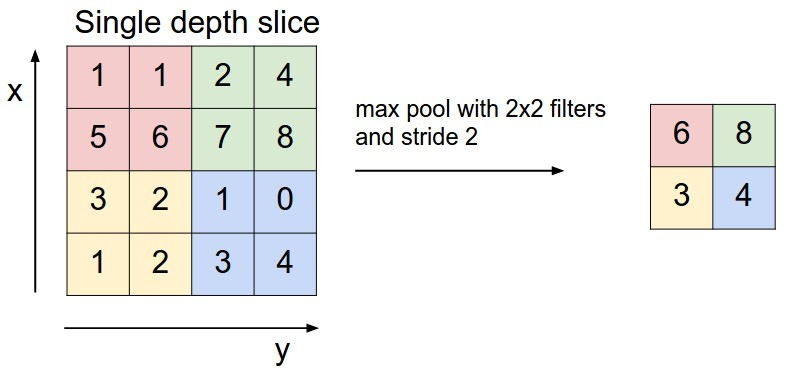
\includegraphics[scale=0.38]{maxpool.jpeg}\end{center}
		\caption[Vrstva združovania - príklad vzorkovania]{Príklad vrstvy združovania, pri ktorom sa rozvzorkuje výstup z konvolučnej vrstvy o veľkosti 4x4, filtrom 2x2, s krokom veľkosti 2 za použitia operácie MAX}\label{fig:cnn}
	\end{figure}
	Takýchto konvolučných vrstiev s vrstvami združovania môže byť aj viac, nemusia ani nutne nasledovať po sebe. Po týchto vrstvách nasleduje plne prepojená vrstva alebo vrstvy (z angl. fully-connected layers), čo je vrstva, v ktorej majú neuróny plné spojenie so všetkými aktiváciami v predošlej vrstve, rovnako ako pri bežných neurónových sieťach. Aktivačnou funkciou neurónov na tejto vrstve býva väčšinou ReLU. Po plne prepojenej vrstve (vrstvách) už nasleduje iba výstupná vrstva. Na obrázku\footnote{https://ujjwalkarn.me/2016/08/11/intuitive-explanation-convnets/} nižšie je jednoduchý náčrt vyššie popísané konvolučnej neurónovej siete. 
	\begin{figure}[H]
		\begin{center}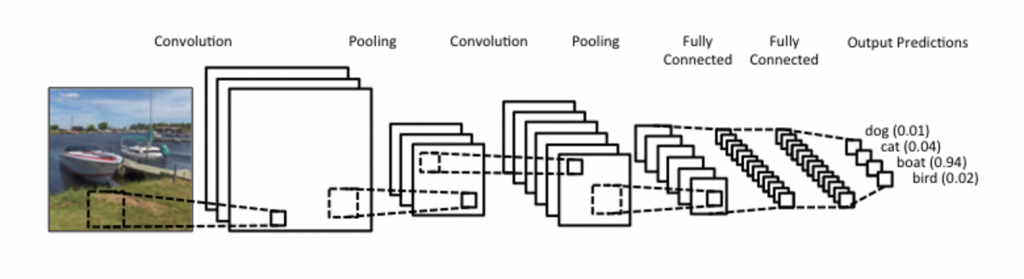
\includegraphics[scale=0.38]{cnn.png}\end{center}
		\caption[Konvolučná neurónová sieť]{Príklad konvolučnej neurónovej siete}\label{conv_nn}
	\end{figure}
	
	Využite tohto typu je v podstate všade, kde sa pracuje s obrázkami. Či už ide o automatické vyznačenie tvárí pre označenie na facebook-u, autonómne vozidlá, ktoré sa vedia riadiť sami (autopilot) alebo triedenie uhoriek na farmách v Japonsku\footnote{https://cloud.google.com/blog/big-data/2016/08/how-a-japanese-cucumber-farmer-is-using-deep-learning-and-tensorflow}. Na tento konkrétny softvér bol použitý príklad kódu jednoduchej konvolučnej siete z tutoriálu\footnote{https://www.tensorflow.org/versions/0.6.0/tutorials/mnist/pros/index.html} pre TensorFlow (knižnica pre prácu s neurónovými sieťami, popísaná v kapitole \ref{tf}), s modifikáciou konvolučnej a združovacej vrstvy tak, aby bola sieť uspôsobená počtu tried uhoriek (10) a ich formátu obrázkov. 
	
	Z mnohých pokusov o autonómnu jazdu stoja za zmienku hlavne tie od Tesly a Google. Prototyp autonómneho systému vozidla od Google-u Dave-2\cite{google_car} využíva model neurónovej siete s 9 vrstvami, jednu normalizačnú, 5 konvolučných a 3 plne prepojené vrstvy. Kamerami spracovaný obraz okolia s frekvenciou 10 snímkov za sekundu (tak nízky počet preto, aby sa predišlo veľkému množstvu príliš podobných obrázkov) je po jednom snímku rozdelený do YUV\footnote{farebný priestor používaný vo video aplikáciách} úrovní a posunutý do neurónovej siete.   
 
\subsubsection{Autoenkóder}
\label{autoencoder}
Autoenkóder (z angl. autoencoder) je špeciálnym typom neurónovej siete, tradične je používaný ako algoritmus učenia bez učiteľa. K učenia však požíva štandardný algoritmus spätného šírenia chyby, kedy sú ale cieľové hodnoty rovné tým vstupným, snaží sa teda naučiť funkciu:
\begin{equation}
	y^{(i)} = x^{(i)}
\end{equation}

Jeho cieľom je v podstate naučiť sa enkódovanú reprezentáciu dát, čo sa využíva napríklad pri komprimácii alebo k zníženiu dimenzionality dát\cite{autoencoder_dimensionality}. Autoenkóder sa skladá z dvoch častí (ako je to vidieť na obrázku \ref{autoencoder_graph}):
\begin{itemize}
	\item enkóder - prvá časť, postupne sa od vstupnej vrstvy zmenšuje počet neurónov, čo v podstate komprimuje vstupnú informáciu do enkódovanie reprezentácie
	\item dekóder - druhá časť, jeho vstupom je práve enkódovaná reprezentácia dát a jeho cieľom je z tejto reprezntácie zrekonštruovať pôvodné dáta
\end{itemize}
 
\begin{figure}[H]
	\begin{center}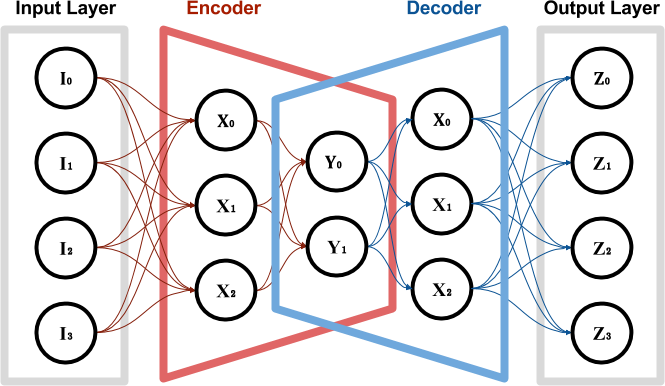
\includegraphics[scale=0.4]{autoencoder.png}
		\caption[Príklad jednoduchého autoenkóderu]{
			Diagram reprezentujúci jednoduchý autoenkóder\footnotemark
		}\label{autoencoder_graph}
	\end{center}
\end{figure}

\footnotetext{https://www.alanzucconi.com/2018/03/14/an-introduction-to-autoencoders/}

I keď cieľom je na konci mať na výstupnej vrstve dokonale zrekonštruovaný vstup, bohužiaľ to tak takmer nikdy nie je a pri autoenkóderoch sa tak jedná o stratovú kompresiu. Zatiaľ nie sú široko rozšírené a v praxi sa používajú najmä pri odstraňovaní šumu\cite{autoencoder_denoising} z dát alebo pri znižovaní ich dimenzionality. Uplatnenie tak nachádzajú hlavne pri spracovaní jazyka\cite{autoencoder_nlp} a počítačovom videní - napríklad pri detekcii objektov\cite{autoencoder_artur}.
 
\subsection{Framework-y pre prácu s neurónovými sieťami}
V dnešnej dobe moderného internetu a dostupnosti technológií máme možnosť výberu z dostatočného množstva framework-ov pre potreby riešenia najrôznejších problémov neurónovými sieťami. Pri výbere môžeme brať do úvahy napríklad preferencie operačného systému (Windows, Linux, ...), programovacieho jazyka (Python, C++, Java, ...), ale aj benefity distribuovaného riešenia a omnoho viac. V nasledujúcich podkapitolách sú preto popísané niektoré z najpoužívanejších technológií pre implementovanie neurónových sietí. 

\subsubsection{TensorFlow}
\label{tf}
TensorFlow\footnote{https://www.tensorflow.org/} je open-source softvérová knižnica, ktorá pre numerické výpočty používa graf dátového toku, kde uzly grafu reprezentujú matematické operácie a hrany multidimenzionálne dátové polia, tzv. tenzory. Graf je možné skonštruovať použitím jazykov s podporou frontend-u (C++, Python, ...). 

Flexibilná architektúra umožňuje vykonávať výpočty na CPU alebo GPU (nepomerne rýchlejšie) na serveroch, desktopových počítačoch či dokonca aj mobilných zariadeniach. Pôvodne bol TensorFlow vyvinutý výzkumníkmi a inžiniermi v Google-i pre strojové učenie a hlboké učenie, avšak jeho využitie je oveľa širšie. V súčasnosti používa TensorFlow veľké množstvo programov, napríklad Google vyhľadávač, prekladač alebo YouTube. 

Momentálne podporuje jazyky C++, Python, Java, Go, Swift.

Medzi hlavné výhody patrí:
\begin{itemize}
	\item podpora pre jednoducho naučiteľné jazyky (Python)
	\item použtie výpočtovej grafovej abstrakcie
	\item vizualizácie pomocou TensorBoard-u\footnote{https://www.tensorflow.org/programmers\_guide/summaries\_and\_tensorboard} (interaktívne grafy pre priebeh učenia, pre model siete, ...)
	\item dostatočne nízko-úrovňový pre plnú kontrolu a implementáciu vlastnej (novej nie len preddefinovanej) funkcionality (v porovnaní napríklad s framework-om Keras (kapitola \ref{keras}))
\end{itemize}

Ako nevýhody možno uviesť:
\begin{itemize}
	\item nedostatok predtrénovaných modelov
	\item pri použití s určitými jazykmi (Python, Java, ...) je pomalý, nakoľko sa nejedná najrýchlejšie jazyky
\end{itemize}

\subsubsection{Microsoft CNTK}
Označuje knižnicu Microsoft Cognitive Toolkit\footnote{https://docs.microsoft.com/en-us/cognitive-toolkit/}, ktorá zlepšuje modularizáciu a údržbu separácie výpočtových sietí, zároveň postkytuje algoritmy učenia a popisy modelov. Má sa jednať o odpoveď na TensorFlow, poskytovaná funkcionalita je veľmi podobná, avšak je o niečo rýchlejší. Princíp a celá architektúra sú zachytené na diagrame na obrázku \ref{cntk_image}. 

\begin{figure}[H]
	\begin{center}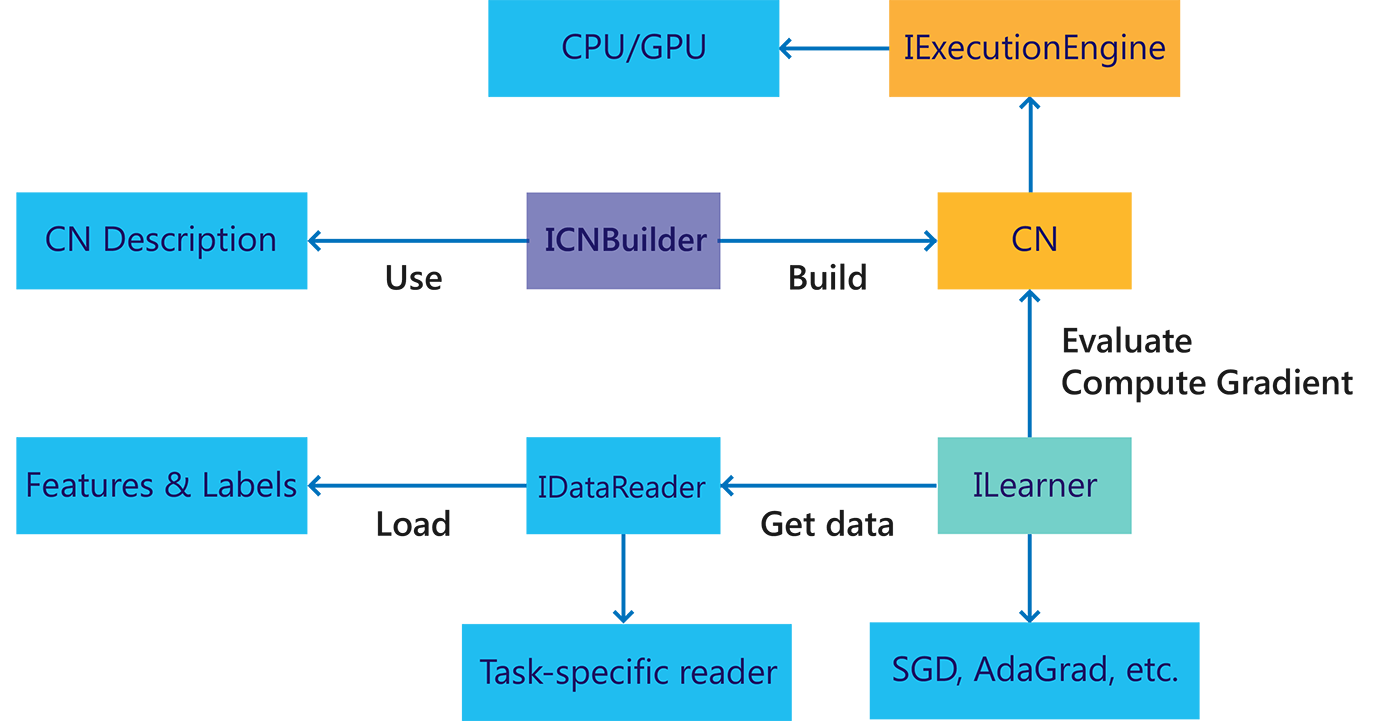
\includegraphics[scale=0.3]{microsoft-cntk-architecture.png}
		\caption[Architektúra fungovania Microsoft CNTK]{
			Diagram zobrazujúci architektúru fungovania Microsoft CNTK\footnotemark
		}\label{cntk_image}
	\end{center}
\end{figure}
\footnotetext{https://dzone.com/articles/progressive-tools10-best-frameworks-and-libraries}

Momentálne podporuje jazyky C++, C\#, Python, Java.

Výhodami tohto framework-u sú:
\begin{itemize}
	\item flexibilita
	\item umožňuje distribuovaný tréning
\end{itemize}

Medzi nevýhody možno zaradiť:
\begin{itemize}
	\item implementácia v novom jazyku, Network Description Language (NDL)
	\item nedostatok možností a nástrojov pre vizualizácie
\end{itemize}

\subsubsection{Theano}

Theano\footnote{https://github.com/Theano/Theano} je veľmi silná knižnica umožňujúca definovanie, optimalizáciu a evaluáciu numerických operácií nad multidimenzionálnymi poliami s obrovskou efektivitou. Podobne ako TensorFlow, k abstrakcii výpočtov používa grafy, ako možno vidieť na príklade na obrázku \ref{theano_image}.

% theano-data-visualization.png

\begin{figure}[H]
	\begin{center}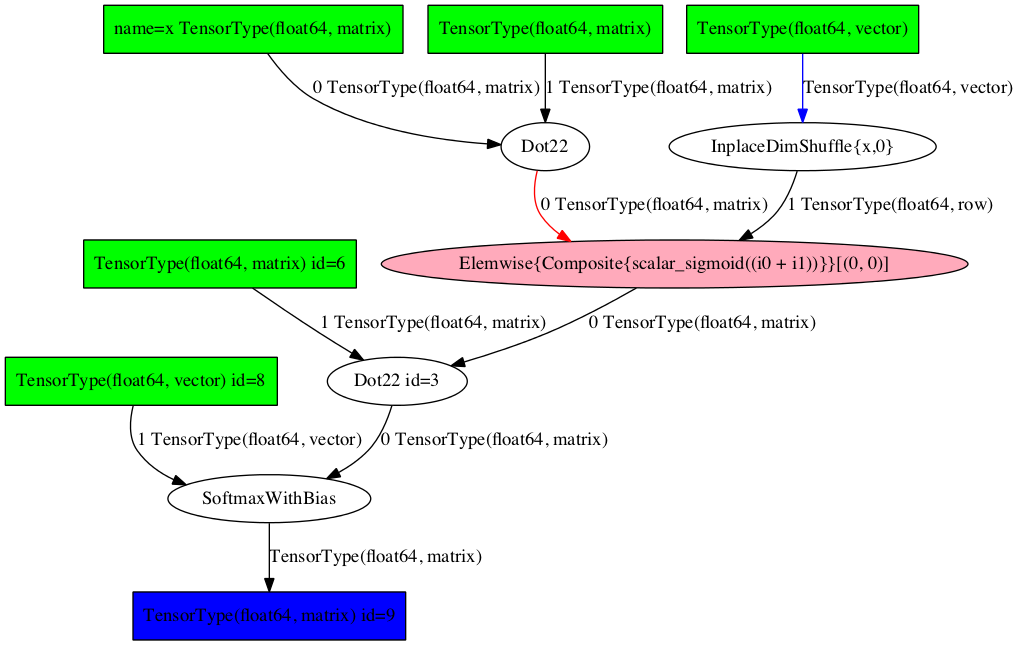
\includegraphics[scale=0.35]{theano-data-visualization.png}
		\caption[Príklad grafovej abstrakcie výpočtov použitím framework-u Theano]{
			Príklad grafovej abstrakcie výpočtov použitím framework-u Theano\footnotemark
		}\label{theano_image}
	\end{center}
\end{figure}
\footnotetext{http://www.wildml.com/2015/09/speeding-up-your-neural-network-with-theano-and-the-gpu/}

Momentálne podporuje iba programovací jazyk Python a v poslednej dobe vývoj tohto framework-u dosť upadá.

Medzi hlavné výhody patrí:
\begin{itemize}
	\item veľmi dobrá optimalizácia pre CPU a GPU (najmä vďaka použitiu nízko-úrovňovej funkcionality naprogramovanej v jazyku C)
	\item vysoko efektívna knižnica pre numerické úlohy
\end{itemize}

Za najväčšie nevýhody sú pokladané:
\begin{itemize}
	\item Theano samo o sebe je v porovnaní s ostatnými knižnicami príliš nízko-úrovňové
	\item potreba použitia s inými knižnicami s vyšším stupňom abstrakcie (napríklad Keras) 
\end{itemize}

\subsubsection{Keras}\label{keras}

Ďalší open-source framework pre prácu s neurónovými sieťami, avšak na rozdiel od predošlých troch nie je vypracovaný ako koncové riešenie pre strojové učenie. Namiesto toho slúži ako rozhranie a poskytuje vyššiu úroveň abstrakcie pre jednoduchšie používanie ostatných framework-ov, z ktorých momentálne pre použitie ako backend podporuje TensorFlow a Theano. Myšlienka stojaca za celým projektom je: \textit{"Byť schopný pretaviť myšlienku na výsledok s čo najmenším zdržaním je kľúčom k dobrému výskum"\footnote{https://keras.io/}}, čo bude aj jedným z dôvodov prečo je práca s ním jednoduchšia.

Keras je v súčasnosti možné používať iba v programovacom jazyku Python.

Jeho hlavnými výhodami sú:
\begin{itemize}
	\item jednoduchosť naučenia, používateľsky veľmi prívetivé
	\item ľahká rozšíriteľnosť
	\item bezproblémový beh aj na CPU aj na GPU
	\item bezproblémové fungovanie aj s Theano-m a aj s TensorFlow-om
	\item rýchle prototypovanie
\end{itemize}

Za jedinú nevýhodu može byť považovaná nemožnosť použitia ako nezávislý framework - vždy je potrebný nejaký ďalší backend.

\subsubsection{Spark MLlib}

Škálovateľná knižnica pre strojové učenie, široko využívaná najmä v distribuovaných systémoch hlavne kvôli svojej efektivite. Veľmi jednoducho je ju môžné pripojiť do Hadoop workflow-u, poskytuje množstvo algoritmov pre strojové učenie optimalizovaných pre výpočty v už spomínaných distribuovaných systémoch na dátach vo veľkom meradle\footnote{https://spark.apache.org/mllib/}.

Momentálne poskytuje podporu pre jazyky Python, Java, Scala a R.

Najväčšími výhodami sú:
\begin{itemize}
	\item vysoká rýchlosť na dátach vo veľkom meradle
	\item dostupnosť v jazykoch, ktoré podobnými framework-ami nie sú často podporované
\end{itemize}

Za nevýhody možno pokladať:
\begin{itemize}
	\item strmá krivka učenia
	\item jednoduché používanie formou "pripoj a hraj" \ (z angl. plug-and-play) dostupné iba pre Hadoop
\end{itemize}

Nevýhodou v porovnaní s vyššie uvedenými framework-ami môže byť nižšie množstvo implementovaných algoritmov, avšak vývoj rozhodne nezaháľa a pridávanej funcionality je stále viac a viac.

\newpage
\null
\thispagestyle{empty}
\newpage

\section{Existujúce modely vizuálnej pozornosti}
\label{saliency_models}
Existujúce modely vizuálnej pozornosti možno z pohľadu typu predikovaných máp výraznosti rozdeliť na modely k predikcii pozornosti zdola nahor \ (kapitola \ref{bottom-up_modely}) a modely k predikcii pozornosti zhora nadol (kapitola \ref{top-down_modely}). Ďalším zaujímavým rozdelením však je rozdelenie podľa použitých princípov a technológií \cite{polatsek}, na modely:

\begin{itemize}
	\item hierarchické - využívajú hierarchické rozkladanie príznakov
	\item Bayesove - využívajú kombináciu výraznosti s predchádzajúcimi znalosťami
	\item rozhodovaco-teoretické - využívajú diskriminačnú teóriu výraznosti
	\item informaticko-teoretické - využívajú maximalizáciu informácie z daného prostredia
	\item grafické - predikcia výraznosti je založená na grafových algoritmoch
	\item vzorovo klasifikačné - využívajú strojové učenie zo vzorov s výraznými črtami
\end{itemize}

\subsection{Modely k predikcii pozornosti zdola nahor}
\label{bottom-up_modely}
Nakoľko práve pozornosť zdola nahor bola prvá skúmaná, existuje k jej predikcii obrovské množstvo najrozličnejších modelov. Niekoľko z nich je popísaných v nasledujúcich podkapitolách. Porovnaním týchto rôznych typov by sa dalo povedať, že ako najlepšie a najpresnejšie sa javia nové moderné postupy strojového učenia. Ich nevýhodou však je potreba dostatočne veľkého datasetu, na ktorom by mohli byť natrénované ako aj značne dlhé trénovanie a predikcie v porovnaní s tými, ktoré používajú rôzne matematické postupy alebo extrakcie čŕt a príznakov, kde fáza trénovania nie je nutná.

\subsubsection{Itti-ho model}

Itti-ho model\cite{itti} je jedným z najznámejších modelov vizuálnej pozornosti, i keď patrí medzi tie staršie, dodnes je široko používaný a citovaný v mnohých článkoch. Je to biologicky inšpirovaný bottom-up model, ktorý využíva hierarchické rozloženie vlastnosí a ich kombináciu do výslednej mapy výraznosti (z angl. saliency map). Ako je vidieť na obrázku \ref{itti_image}, zo vstupného obrázka sa vytvoria 3 typy máp a to podľa farby, intenzity a orientácie, ktorých kombináciou sa dosiahne už spomenutá mapa výraznosti. 

\begin{figure}[H]
	\begin{center}
		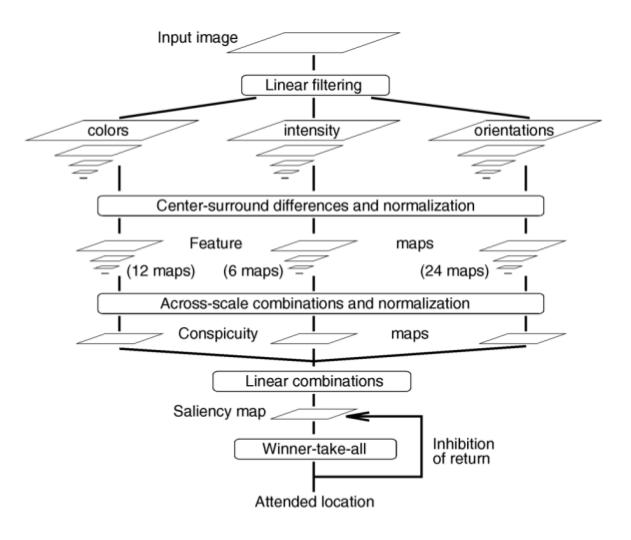
\includegraphics[scale=0.4]{itti_model.jpeg}
	\end{center}
	\caption[Itti-ho hierarchický model vizuálnej pozornosti]{Itti-ho hierarchický model vizuálnej pozornosti\cite{itti}\label{itti_image}}
\end{figure}

\subsubsection{Metóda hierarchickej výraznosti}

Pri použítí metódy hierarchickej výraznosti (z angl. hierarchical-saliency method\cite{gao2013hierarchical}) sa v podstate jedná o detekciu charakteristík v prirodzenej scéne. Tento postup je istým vylepšením predchádzajúceho Ittiho modelu a prakticky pozostáva z nasledujúcich dvoch krokov:

\begin{itemize}
	\item \textit{prvý krok} - extrakcia globálne výrazných oblastí (z angl. globally salient
	regions):
		\begin{enumerate}
			\item výpočet mapy výraznosti \textit{S} zo vstupného obrázka \textit{I}
			\item evaluácia oblastí záujmu (z angl. regions of interest, ROIs), automatická
			klasifikácia všetkých pixelov do dvoch kategórií k získaniu masky \textit{M}:
			\begin{itemize}
				\item[-] globálne výrazné oblasti (\textit{1})
				\item[-] zvyšok (\textit{0})
			\end{itemize}
			\item vynásobenie masky \textit{M} so vstupným obrázkom \textit{I} k získaniu filtrovaného
			obrázka \textit{I'}
		\end{enumerate}
	\item \textit{druhý krok} - evaluácia lokálne výrazných častí vo vnútri globálne výrazných
	oblastí. Použije sa vyfiltrovaný obrázok \textit{I'} z predchádzajúcich krokov k získaniu novej mapy výraznosti \textit{S'}, ktorá je finálnou mapou.
\end{itemize}
	
\subsubsection{Model pre určovanie salientných oblastí webových stránok}

Veľmi zaujímavým riešením pre predikciu a určovanie salientných oblastí scény v doméne webových stránok je model od Chengyao Shen a Qi Zhao\cite{Saliency} využívajúci metódy strojového učenia. Model je postavený na použití metódy MKL (Multiple Kernel Learning - kombinuje viacero jadier SVM (Support Vector Machine) miesto jedného), ktorá bola 
trénovaná na princípe binárneho regresného problému. Rozdiel oproti predošlým popisovaným modelom je však v tom, že predikovaná nebola priamo výsledná mapa výraznosti ale iba vektor pohľadov (fixácií) na vstupné obrázky, na základe ktorého bola potom spomínaná mapa vypočítaná. Autori po vyhodnotení výsledkov zistili že ako najviac salientné oblasti sa v scéne javia v prvom rade ľudská tvár, oči a celkovo vrchná časť ľudského tela. Zaujímavým vylepšením ich modelu však bolo to, že tieto zistenia zapracovali formou predtrénovania MKL na tieto vysoko salientné oblasti. 


\subsection{Modely k predikcii pozornosti zhora nadol}

\label{top-down_modely}
Predikcia pozornosti zhora nadol (top-down) je značne zložitejšia, nakoľko sa do úvahy berie aj sématický kontext scény. Tým môže byť napríklad emočný obsah (kapitola \ref{emotion_content}), či hľadanie konkrétnych objektov v scéne (kapitola \ref{caption_model}).


\subsubsection{Zameranie na emočný obsah}
\label{emotion_content}
Niekoľko riešení sa v posledných rokoch pokúsilo o predikovanie pozornosti zhora nadol (top-down) na základe emočného obsahu v pozorovanej scéne. Z nich stojí za zmienku napríklad model od Liu a spol. \cite{liu2016improving}, ktorí sa zamerali na spomínaný emočný obsah v rôznych oblastiach (blokoch) obrázka, kde do úvahy brali:
\begin{itemize}
	\item emočné objekty, napr. hady a krv (evokujú silný strach)
	\item výrazy tváre
	\item všeobecný emočný obsah
\end{itemize}

Hlavné problémy, ktoré riešili, by sa dali zhrnúť do dvoch otázok:
\begin{itemize}
	\item Ako získať a ohodnotiť intenzitu emócií pre obrázok?
	\item Aký typ emócie by mal byť dominantným pre jednotlivé obrázky?
\end{itemize}

Ich narhované riešenie malo niekoľko častí. Prvou je extrakcia faktorov pozornosti zdola nahor (bottom-up) vo forme nízko-úrovňových máp výraznosti založených na črtách a mapy priestorovej polohy s dôrazom na centrum pre výpočet odhadu hustoty pohľadu (z angl. gaze density estimation). K tomuto boli použité klasické hierarchické modely pre určovanie pozornosti (napr. Itti-ho model).

Druhou časťou je detekcia emócií, k čomu bol použitý emočný detektor založený na učení s použitím učenia viacerých inštancií (z angl. multiple instance learning, MIL) zo slabo oštítkovaných dát. Tými boli obrázky označené emočným typom\footnote{jedna z 8 skupín, do ktorých boli rozdelené emócie. Príkladom týchto skúpín sú napr. hnev, láska, smútok, prekvapenie, atď.}, ktorý bol určený po vypočítaní pravdepodobnosti vyskýtu jednotlivých typov pre každú časť obrázka. Touto matematickou operáciou sa autorom podarilo úspešne vyriešiť problém určenia dominantného typu emócie pre obrázok.  Ďalej bol pre zlepšenie extrakcie emócií použitý mechanizmus založený na SVM, ktoré bolo použité na detekciu ľudských tvárí a odhadnutie intenzity výrazu. Výstupom z tejto časti je emočná mapa, ohodnocujúca intenzitu emócií, určená pre ďalšie spracovanie.

Treťou časťou bolo spracovanie výstupov z predošlých dvoch častí lineárnym SVM, ktoré vo výsledku z faktorov pozornosti zdola nahor (bottom-up) a emočných faktorov vygeneruje výslednú mapu hustoty pohľadu (z angl. gaze density map). Vyššie popísaný postup je zobrazený na diagrame na obrázku \ref{liu_image}.

\begin{figure}[H]
	\begin{center}
		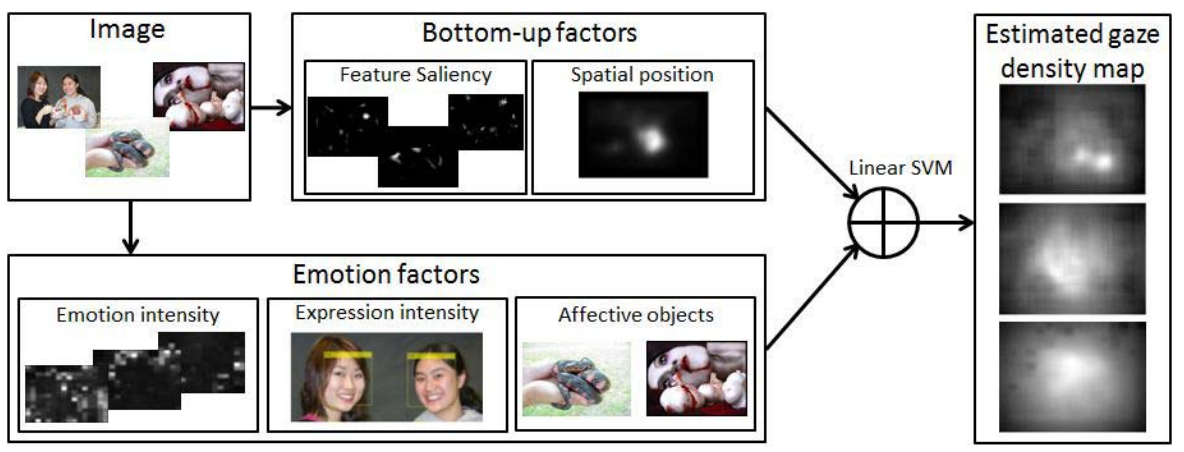
\includegraphics[scale=0.43]{liu_emotion_model.PNG}
		\caption[Diagram modelu k predikcii máp výraznosti založených na emočnom obsahu]{Diagram modelu od Liu a spol. k predikcii máp výraznosti založených na emočnom obsahu\cite{liu2016improving}\label{liu_image}}
	\end{center}
\end{figure}

Za veľkú výhodu tohto riešenia by sa dala pokladať kombinácia viacerých faktorov (aj pozornosti zdola nahor (bottom-up) aj pozornosti zhora nadol (top-down emočné faktory)  do výslednej mapy, vďaka čomu sa viac priblíži k reálnej pozornosti. Ako vieme tú neovplyvňujú čisto len jedny alebo druhé faktory, ale vždy je to ich kombinácia. Ako mierna nevýhoda by sa mohlo javiť rozdelenie emócií iba na 8 typov a určenie ako dominantný typ len jeden z nich, pričom ostatné sa ďalej neberú do úvahy.  

% TODO maybe \subsubsection{CRF}

\subsubsection{SAM}
SAM - skratka pre Saliency Attentive Model\cite{cornia2016predicting}, ďalší z modelov schopných aj predikcie pozornosti zhora nadol (top-down). Založený je na architektúre nazvanej ML-Net (Multi-Level Network\cite{cornia2016deep}), ktorá miesto klasických konvolučných vrstiev využíva dilatované konvolučné vrstvy, ktoré limitujú efekt zmenšovania. Táto architekúra použitá pre spracovanie vstupného obrázka je nasledovaná konvolučnými LSTM vrstvami, ich naučené výstupy potom spracováva už klasická konvolučná vrstva, výstupom ktorej je mapa výraznosti. Popisovaný postup je zobrazený na obrázku \ref{dilated_model_image}.

\begin{figure}[H]
	\begin{center}
		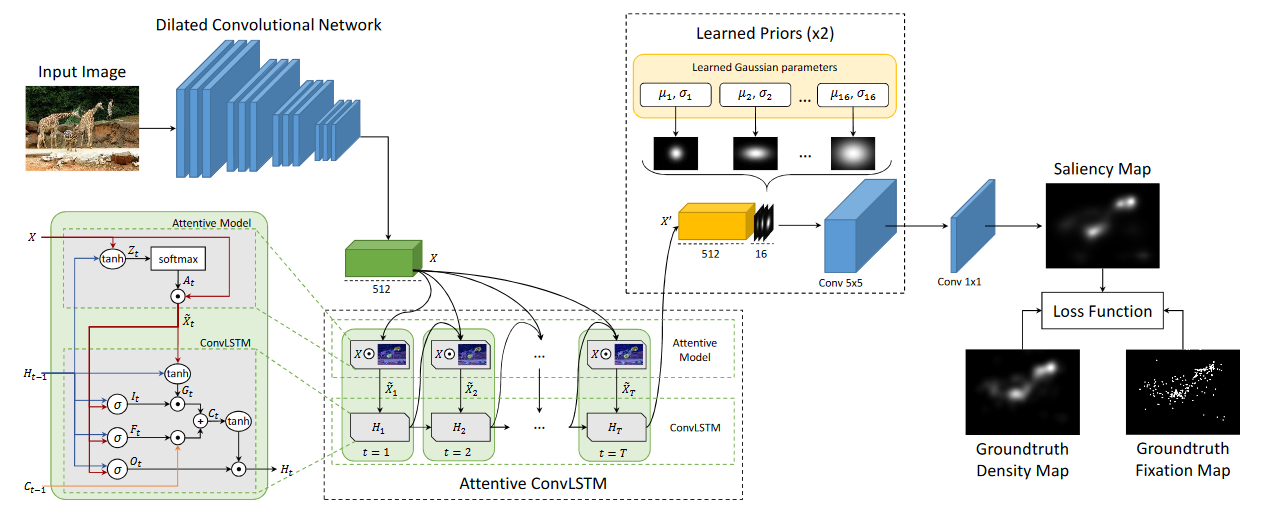
\includegraphics[scale=0.41]{dilated_NN.PNG}
		\caption[Diagram konvolučnej LSTM siete]{Diagram modelu využívajúceho dilatované konvolučné vrstvy v kombinácii s LSTM vrstvami \cite{cornia2016predicting}\label{dilated_model_image}}
	\end{center}
\end{figure}

Vďaka architektúre zobrazenej na obrázku vyššie je možné nezávisle na sebe trénovať dilatovanú konvolučnú sieť (alebo použiť predtrénovanú, či o niečo inú) a konvolučnú LSTM sieť. Veľkou výhodou dilatovanej konvolučnej siete je stratégia zväčšenia výstupného rozlíšenia obrázka, zatiaľ čo sa zachováva mierka, na ktorej operujú konvolučné filtre a počet parametrov. To je rozdiel oproti klasickej konvolučnej sieti, kedy je vstupný obrázok po extrakcii čŕt obvykle zmenšený, čo môže značne zhoršiť presnosť predikcie máp výraznosti.

Spomínané LSTM vrstvy (podrobnejšie zobrazené aj na obrázku \ref{dilated_model_image}) využívajú kombináciu aktivačných funkcií \textit{softmax}, \textit{tanh} a \textit{sigmoid}, kedy pri spracúvaní sekvenčne aktualizujú svoj interný stav. Ako vstup dostanú vektor extrahovaných čŕt z dilatovaných konvolučných vrstiev (\textit{X}), ktoré spracúvajú vstupné obrázky, a generovanú mapu výraznosti z predošlej LSTM vrstvy (s výnimkou prvej). Táto generovaná mapa je ešte upravená mechanizmami pozornosti, ktoré sa selektívne zameriavajú na rôzne časti obrázku. Vo výsledku je potom vektor extrahovaných čŕt (\textit{X}) a upravená generovaná mapa (\textit{$X_t$}) z predošlej vrstvy ešte ďalej spracovávaná aktovačnými funkciami \textit{tanh}.

Výstup z týchto vrstiev je ďalej upravený štandardnými konvolučnými vrstvami do výsledných máp výraznosti.

Ďalšou zaujímavou vecou na tomto riešení je zvolenie funkcie chyby (z angl. loss function). Autori nepoužili žiadny z tradičnejších typov, ale použili lineárnu kombináciu troch rôznych evaluačných metrík (popísané v kapitole \ref{metric}), v tvare:

\begin{equation}
	L (y, y^{den}, y^{fix}) = \alpha L1(y, y^{fix}) + \beta L2(y, y^{den}) + \gamma L3(y, y^{den})
\end{equation}

Pre vyššie uvedené platí:

$y$ - predikovaná mapa výraznosti

$y^{den}$ - pravdepodobnostná distribúcia (z angl. groundtruth density distribution)

$y^{fix}$ - binárna mapa fixácií

$\alpha, \beta, \gamma $ - tri skalárne hodnoty určené k vybalancovaniu troch funkcií chyby

$L1, L2, L3$ - tri funkcie pre výpočet evaluačných metrík, za radom Normalizovaná cesta výraznosti (NSS, z angl. Normalized Scanpath Saliency), Lineárny korelačný koeficient (CC), Kullback-Leiblerova divergencia (KL-Div), všetky bližšie popísané v kapitole \ref{metric}.

Za veľkú výhodu tohto riešenia pokladáme možnosť predikcie aj oboch typov pozornosti, v závislosti od datasetu, na ktorom je model natrénovaný. Taktiež možnosť nezávislej výmeny submodelov (dilatovaná konvolučná sieť,  konvolučná LSTM sieť) sa javí ako veľmi výhodná, keďže uľahčuje protypovanie bez nutnosti nového natrénovania celého modelu. Za miernu nevýhodu možno považovať značnú komplexitu modelu a s tým spojené nároky na hardvér, rovnako ako aj na čas nutný na natrénovanie od nuly, v prípade, že nechceme použiť predtrénované modely. 

\subsubsection{Pozornosť zhora nadol vedená titulkami}
\label{caption_model}
Jedným z ukážkových príkladov pozornosti zhora nadol (top-down) je úloha nájdenia nejakého konkrétneho objektu v scéne, čím sa inšpirovali výskumníci z Bostonskej univerzity. Predstavili model\footnote{http://ai.bu.edu/caption-guided-saliency/} \cite{ramanishka2017top} schopný predikcie máp výraznosti na základe kľúčových slov v zadanej vete a príslušnom obrázku alebo videu, príklad predikcií možno vidieť na obrázku \ref{top_down_captions_image}.

\begin{figure}[H]
	\begin{center}
		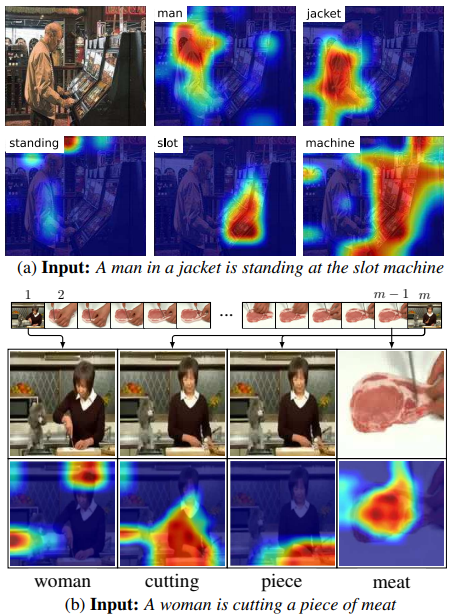
\includegraphics[scale=0.7]{top_down_captions.PNG}
		\caption[Predikcia salientných oblastí na základe kľúčových slov vo vete]{Predikcia salientných oblastí na základe kľúčových slov vo vete, hore po \textbf{a} predikcia pre obrázok, dolu po \textbf{b} predikcia pre video\cite{ramanishka2017top}\label{top_down_captions_image}}
	\end{center}
\end{figure}

Autori použili prístup nazvaný titulkami vedená vizuálna pozornosť (z angl. Caption-Guided Visual Saliency), ktorý produkuje mapy výraznosti pre nepohyblivé obrázky alebo video. Ako základný model použili LSTM enkóder-dekóder (z angl. encoder-decoder), ktorý predikuje aj dočasné (z videa) aj priestorové (z obrázkov) salientné mapy na základe kľúčových slov vo vete (vstupné titulky, popis) a mapuje ich na vstupné obrázky (alebo video). Vstupné titulky sú spracovávané LSTM vrstvami. Na obrázku \ref{top_down_captions_model_image} je možné vidieť načrtnutý model riešenia. Ako prvá vstupná vrstva funguje konvolučná neurónová sieť reprezentujúca enkóder pre video, ktorá "zakóduje" \ reprezentáciu obrázkov aj s aktiváciami všetkých vizuálnych konceptov detekovaných vo videu. Tieto informácie posunie ďalej ako vektor pre LSTM vrstvy reprezentujúce dekóder - ten rozhoduje o tom, ktoré časti použije pomocou LSTM výstupných brán k predikcii mapy výraznosti pre kľúčové slovo v čase \textit{t}. Autori ďalej zvolili veľmi šikovné riešenie pre predikciu máp len pre obrázky - jednoducho výstup produkovaný poslednou konvolučnou vrstvou zmenili na tzv. "dočasnú" sekvenciu (vektor): $V = (v_1, . . . , v_m)$. Tá je vytvorená sekvenčne scan-ovaním obrázka riadok po riadku z ľavého horného rohu do pravého dolného rohu. Prvá LSTM vrstva potom tento upravený vektor spracuje a posunie ďalej k dekódovaniu na kľúčové slová vo vete.

\begin{figure}[H]
	\begin{center}
		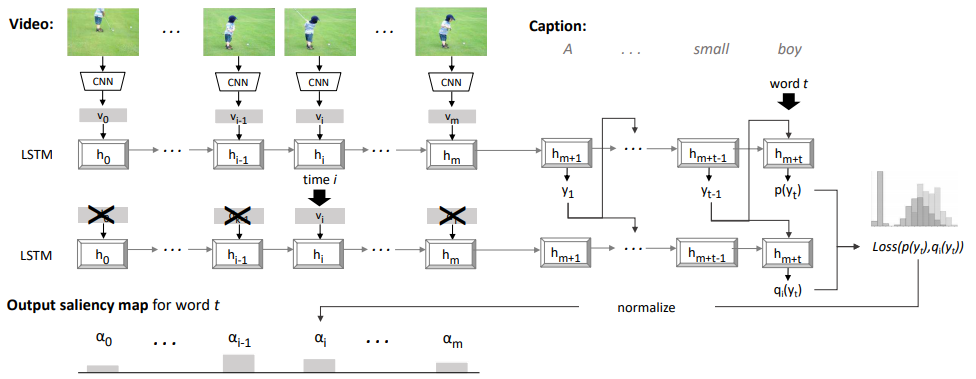
\includegraphics[scale=0.52]{top_down_captions_NN.PNG}
		\caption[Model neurónovej siete pre predikciu na základe kľúčových slov]{Diagram modelu neurónovej siete\cite{ramanishka2017top}, zhora vstup vľavo vo forme videa, vpravo titulky k nemu. V strede LSTM vrtvy neurónovej siete, dolu výstupná mapa výraznosti pre kľúčové slová. \label{top_down_captions_model_image}}
	\end{center}
\end{figure}

Popisované riešenie je ukážkovým modelom pre predikciu pozornosti počas hľadania objektov v scéne. Veľkou výhodou je použitie LSTM vrstiev pre zachytenie predošlého kontextu ako aj možnosť predikcie pre video aj obrázky iba s minimálnymi zmenami.

\subsection{Detekcia objektov}
\label{object_detection}
Z pohľadu modelov vizuálnej pozornosti môžu za zmienku stáť aj modely pre detekciu objektov a ich klasifikáciu, ktorých je dostupné značné množstvo aj predtrénovaných. Ako príklad si môžeme uviesť konvolučnú sieť VGG-Net\cite{vgg_net} určenú práve pre klasifikáciu objektov na obrázku. Skladá sa z 16 konvolučných vrstiev a veľkého množstva filtrov, ako možno vidieť na obrázku \ref{vgg_net_model}. Spracováva obrázky o veľkosti \textit{224x224}, bola trénovaná na 4 GPU 2-3 týždne a skladá sa zhruba zo 138 miliónov parametrov\footnote{https://medium.com/@sidereal/cnns-architectures-lenet-alexnet-vgg-googlenet-resnet-and-more-666091488df5}.  Je častou voľbou pre ďalšie experimentovanie v oblasti pre svoju presnosť a dostupnosť už natrénovaného modelu.

\begin{figure}[H]
	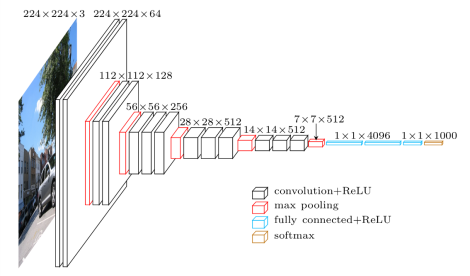
\includegraphics[scale=0.8]{vgg_net.png}
	\caption[VGG-Net]{Štruktúra neurónovej siete VGG-Net\footnotemark}\label{vgg_net_model}
\end{figure}

\footnotetext{https://www.quora.com/What-is-the-VGG-neural-network}

Ďalším zaujímavým riešením detekcie objektov v obrázku je autoenkóder od A. Meyer-a\cite{autoencoder_artur}, ktorý využíva aj vyššie popisovanú sieť VGG-Net. Využil princíp konvolúcie-dekonvolúcie kedy práve VGG-Net funguje ako enkóder a jej v podstate zrkadlová podoba s dekonvolučnými vrstvami funguje ako dekóder (zobrazené na obrázku \ref{autoencoder_artur_graph})

\begin{figure}[H]
\centering	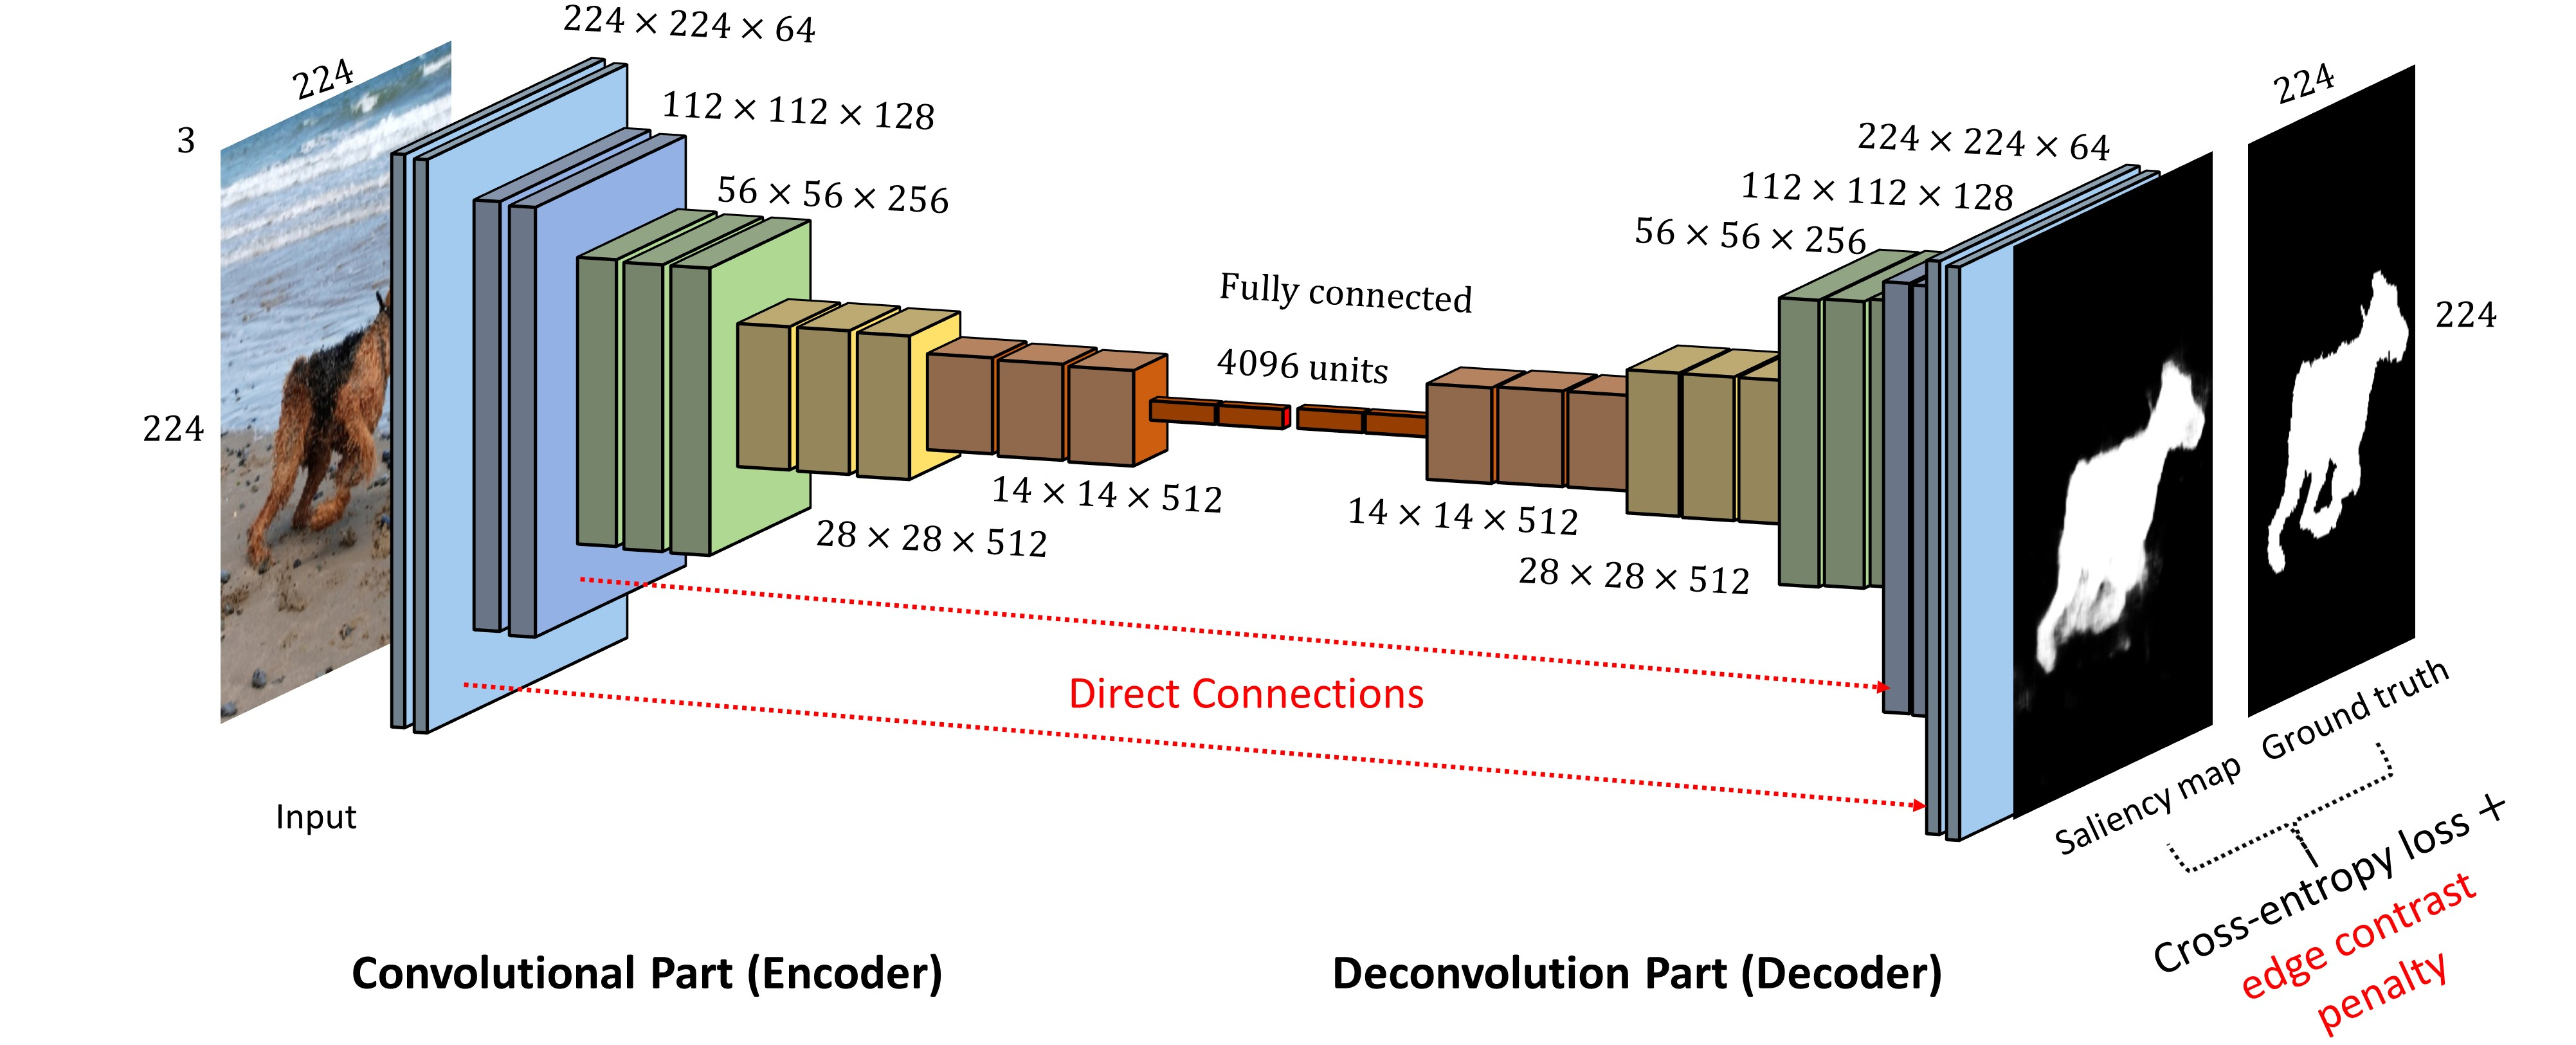
\includegraphics[scale=0.12]{autoencoder_artur.jpg}
	\caption[Autoenkóder pre detekciu objektov]{Štruktúra autoenkóderu pre detekciu objektov\footnotemark}\label{autoencoder_artur_graph}
\end{figure}

\footnotetext{https://github.com/arthurmeyer/Saliency\_Detection\_Convolutional\_Autoencoder}

Sieť je schopná aj priamych prepojení z konvolučných do dekonvolučných vrstiev a predikuje v podstate binárny obrázok, kde hodnota 1 reprezentuje pixel nájdeného objektu. Veľkou výhodou pri takejto sieti je možnosť použitia predtrénované modelu VGG-Net-u pre enkóder. 


\newpage
\null
\thispagestyle{empty}
\newpage


\section{Metriky používané na ohodnotenie modelov vizuálnej pozornosti}
\label{metric}

Obvykle sa modely k predikcii vizuálnej pozornosti evaluujú 2 spôsobmi, a to buď vzhľadom na pohyb očí (resp. fixácie) alebo vzhľadom na originálnu mapu výraznosti. K tomu slúži veľké množstvo metrík\cite{metriky}, medzi tie najčastejšie používané patria:

\begin{itemize}
	
	\item NSS - Normalizovaná cesta výraznosti (z angl. Normalized Scanpath Saliency). Využíva priemer hodnôt výraznosti na \textit{n} fixácií v normalizovanej mape podľa nasledovného vzorca: 
	
	\begin{equation}
	\frac{1}{n} \sum_{i=1}^{n} \frac{s(x_{h}^{i}, y_{h}^{i}) - \mu_{s}}{\sigma _{s}}
	\end{equation}
	
	\item AUC - Oblasť pod ROC krivkou (z angl. Area Under the ROC Curve).
	Ľudské fixácie sú považované za pozitívnu sadu a niektoré body na obrázku sú vybrané ako negatívna sada. K mape výraznosti je potom pristupované ako k binárnemu klasifikátoru na separáciu pozitívnych vzorkov od negatívnych. Presnosť podľa tejto metriky je daná nasledovne: 
	
	\begin{itemize}
		
		\item 0.90 - 1 = výborná
		\item 0.80 - 0.90 = dobrá
		\item 0.70 - 0.80 = priemerná
		\item 0.60 - 0.70 = slabá
		\item 0.50 - 0.60 = veľmi slabá
		
	\end{itemize}
	
	\item sAUC - Zamiešaná oblasť pod ROC krivkou (z angl. shuffled Area Under the ROC Curve) je mierna modifikácia vyššie uvedenej metriky, kedy ako negatívna sada nie sú vybrané len niektoré body, ale všetky body, ktoré nie sú ľudskými fixáciami, sú považované za negatívne. Určenie presnosti na základe hodnôt je rovnaké ako pri AUC. 
	
	\item CC - Korelačný koeficient, určuje prakticky podobnosť v tomto prípade dvoch máp výraznosti, kde jedna je výsledok modelu vizuálnej pozornosti a druhá je reálna mapa vypočítaná z fixácií. 
	
	\begin{equation}
	CC (s, h) = \frac{cov(s, h)}{\sigma_{s} \sigma _{h}}
	\end{equation}
	
	\item KL-Div - Kullback-Leiblerova divergencia\cite{bylinskii2016different}, všeobecné teoretické meranie rozdielu medzi dvoma pravdepodobnostými distribúciami. V oblasti predikcií vizuálnej pozornosti sa často nazýva aj AUC-Judd. Ako vstup berie mapu výraznosti \textit{P} a mapu fixácií (z angl.  ground  truth  fixation map) \textit{$Q^{D}$}, evaluuje stratu informáciie keď je \textit{P} použité k aproximácii \textit{$Q^{D}$}.
	
	\begin{equation}
		KL (P, Q^D) =  \sum_{i} Q_{i}^{D} log \left ( \epsilon + \frac{Q_{i}^{D}}{\epsilon + P_i} \right )
	\end{equation}
	
\end{itemize}
 
 
% ----------------------------------------------------------------------------------------
\iffalse	
\subsection{Určenie pútavých častí webových stránok pomocou strojového učenia}
\label{machine_learning}
	V nasledujúcej časti sú opísané niektoré z existujúcich riešení problému určenia pútavých častí grafického rozhrania webovej stránky za použitia strojového učenia. V podstate existujú 2 prístupy, z ktorých jeden vychádza z HTML kódu stránku a druhý len z jej obrázku, screenshot-u. 
	

\subsubsection{Riešenia na báze segmentácie stránok}

	Tento spôsob na začiatku vyhádza z HTML kódu stránky, ktorú na jeho základe rozdelí tzv. segmentovaním na hlavné časti (segmenty, bloky) stránky. Segmentácia používa buď segmentačné algoritmy na rozdelenie stránky do blokov podľa rôznych vlastností, alebo používa dátové štruktúry na reprezentáciu komponentov a elementov HTML dokumentu. 
    Najpoužívanejšie prístupy k segmentácii sú:
\begin{my_itemize}
	\item {Segmentácia založená na DOM\cite{DOM} (dokumentový objektový model, z angl. document object model):}
	\newline
\hspace{10mm}HTML dokument je reprezentovaný ako DOM strom. Tagy môžu reprezentovať jeden blok stránky, napr. P-paragraf, TABLE-tabulka, atď. I keď tento strom dokáže veľmi presne reprezentovať štruktúru HTML dokumentu (stránky), často nie je dostatočne presný pri 	rozdelení sémanticky (vizuálne) rôznych blokov. 
	\item {Segmentácia založená na lokácii\cite{block_importance} (z angl. location-based segmentation):}
	\newline
\hspace{10mm}Stránka sa rozdelí na 5 hlavných častí: stred, vľavo, vpravo, hore, dolu. Problémom je však, že nie vždy sa toto rozdelenie hodí na každú stránku a v prípade, že je stránka príliš dlhá (scroll-ovateľná) sa časti, ktoré boli na začiatku napr. dolu, posunú smerom hore a rozdelenie stránky sa tým zmení. 
	\item {VIPS\cite{vips} - segmentácia stránky založená na pohľade (z angl. vision-based page segmentation):}
	\newline
\hspace{10mm}VIPS je v podstate kombinácia predchádzajúcich dvoch algoritmov. Delí stránku aj na základe farby, veľkosti blokov atď. V prvom rade vyberie vhodné uzly z DOM stromu a nájde medzi nimi separátory, ktoré naznačujú horizontálne a vertikálne línie webovej stránky. Na základe DOM stromu a separátorov sa vytvorí sémantický strom stránky, v ktorom je každý segment stránky reprezentovaný ako samostatný uzol v strome, koreňom stromu je samotná stránka. Spojitosť segmentácie stránky je kontrolovaná prededifinovaným stupňom koherencie ( z angl. Predefined Degree of Coherence (PDoC\cite{PDOC})) – každému uzlu je daný určitý stupeň súvislosti, čo zabezpečuje, že VIPS dokáže efektívne držať obsah pokope, zatiaľ čo sémanticky odlišné bloky od seba.
\end{my_itemize}

	Ako príklad riešenia používajúceho spomínanú segmentáciu je možné uviesť prácu výskumníkov z Microsoftu \cite{block_importance}. Tí použili VIPS algoritmus na segmentovanie a 5 ľudí, ktorí manuálne oštítkovali každý blok webovej stránky. Bloky sú očíslované od 1 po 4 podľa dôležitosti (1 – nepodstatné informácie ako reklamy, 4 – najdôležitejšia časť stránky, hlavný obsah). Z nich sa potom zostrojí model dôležitosti blokov, čo je vlastne funkcia mapovania každého bloku a jeho dôležitosti zobrazená ako:    
	\begin {center}
	\center \{ block features \} → block importance
	\newline
	\end {center}

	Vizualizácia mapovania dôležitosti blokov je zobrazená na časti stránky na obrázku \ref{fig:cnn_rbf}.

		\begin{figure}[H]
			\begin{center}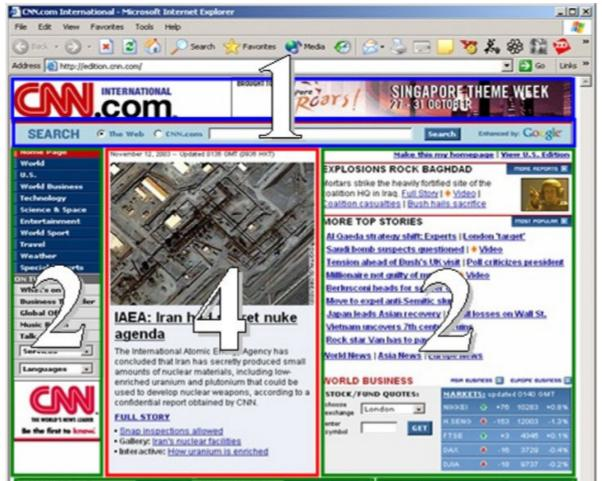
\includegraphics[scale=0.3]{cnn_rbf.jpeg}\end{center}
			\caption[Vizualizácia mapovania dôležitosti blokov webových stránok]{Vizualizácia mapovania dôležitosti blokov webových stránok\cite{block_importance}. 1 - najmenej dôležité informácie, 4 - najpodstatnejšia časť stránky}\label{fig:cnn_rbf}
		\end{figure}

	Na odhad dôležitosti blokov sa potom nahliada ako na regresný problém a na jeho riešenie je  použitá neurónová sieť, v ktorej sú bloky reprezentované ako dvojica (\textit{x, y}), kde \textit{x} je reprezentácia bloku a \textit{y} je dôležitosť (berie sa ako reálne číslo).  Typ siete je RBF (radial basis function) a vyhľadávacou technikou je štandardný gradient descent. Sieť zahŕňa 3 vrstvy, každú s inou funkciou. Prvú (vstupnú) vrstvu tvoria zdrojové uzly, druhá je jediná skrytá vrstva a zabezpečuje nonlineárnu transformáciu zo vstupného priestoru do skrytého. Obsahuje RBF neuróny, ktoré kalkulujú vstup skrytej vrstvy kombináciou vážených vstupov a odhadov. Tretia (výstupná) vrstva dodáva dôležitosť blokov do reprezentácie blokov aplikovanej v prvej (vstupnej) vrstve. 
	
	Výhodou tohto riešenia je rozdelenie stránky podľa logických blokov, nevýhodu vidím v začiatočnom ohodnotení blokov ľuďmi podľa dôležitosti, pretože mi to príde príliš individuálne. Tiež rozdelenie stránky do stromu s jednotlivými blokmi a časťami je v závislosti od stránky dosť pamäťovo náročná operácia. 
	
\subsubsection{Riešenia vychádzajúce z obrázku stránky}
\label{singapur}
	Tento typ riešenia používa k určeniu dôležitých (pútavých) častí stránky jej screenshot. Autormi modelu sú Chengyao Shen a Qi Zhao\cite{singapur_model}. Tí na začiatku rozdelili ich dataset do niekoľkých kategórií podľa obsahu stránky, t. j. ilustrované (prevládajú obrázky), textové (prevažne blogy, články, atď.) a mix predošlých dvoch kategórií. V každej z nich bolo približne 50 obrázkov s rozlíšením 1360x768. Na obrázky web stránok  potom pozeralo 11 subjektov a ich sekvencie pohľadov boli zaznamenané pomocou MATLABU s Psychtoolbox\cite{psych} a systémom Eyelink 1000.
	
	Na predikciu pohľadov\cite{saliency} na web stránky bola použitá metóda MKL (Multiple Kernel Learning - kombinuje viacero jadier SVM\footnote{Support Vector Machine - modely učenia s príslušnými algoritmami učenia, ktoré analyzujú dáta použité pre klasifikáciu a regresnú analýzu\cite{SVM}} miesto jedného). MKL bolo trénované ako binárny regresný problém, z datasetu bolo použitých 119 obrázkov na trénovanie, zvyšných 30 bolo použitých na finálne testovanie. Predikovaný bol vektor pohľadov (fixácií) na obrázok. Vyhodnotením datasetu bolo zistené, že človeka mimo iné upúta pri pohľade na web stránku v prvom rade ľudská tvár, oči a celkovo horná časť tela, či neprimerane veľké logo. Taktiež sa dá predpovedať, že človek sa začne pozerať v prvom rade najprv do strednej  oblasti a oblasti viac vľavo hore od stredu. Tieto zistenia dokázali veľmi dobre zapracovať aj do ich modelu. Na obrázku nižšie je možné vidieť vizualizáciu pohľadu na rôzne typy stránok v prvých 5 sekundách formou teplotných máp.
		\begin{figure}[H]
			\begin{center}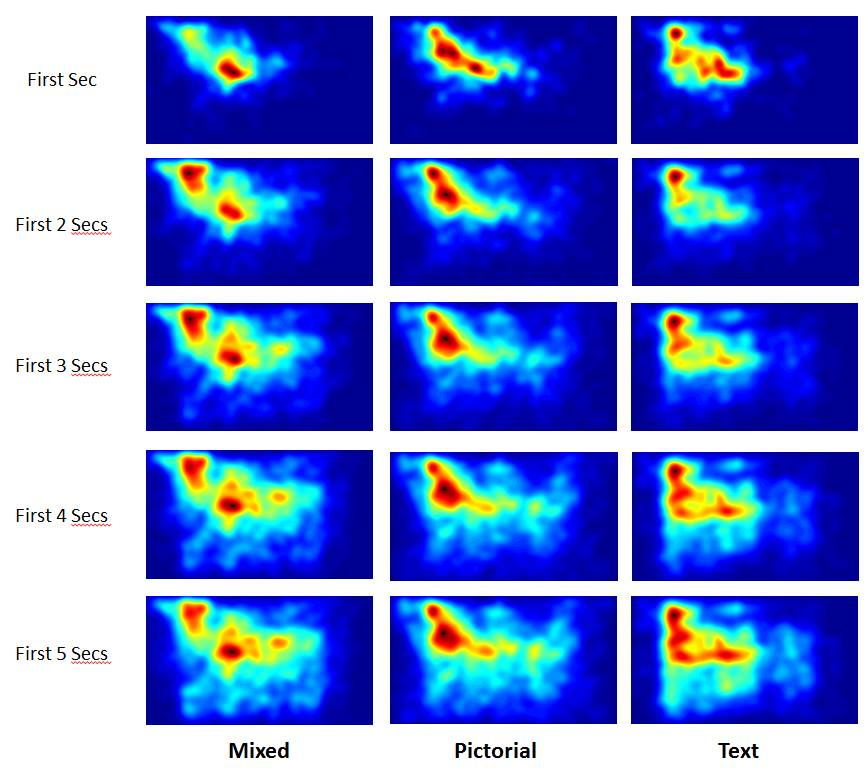
\includegraphics[scale=0.3]{heatmaps.png}\end{center}
			\caption[Vizualizácia pohľadu formou teplotných máp]{Vizualizácia pohľadov v prvých 5 sekundách. Vľavo mix stránok, v strede prevažne ilustrované stránky a vpravo textové.\cite{singapur_model}}%\label{simple_nn}
		\end{figure}
		
	Za výhodu tohto riešenia oproti predošlému pokladám hlavne vygenerovanie heat mapy, ktorá vypovie o dôležitých častiach stránky ďaleko viac ako očíslované HTML bloky. Taktiež zistenia, že človek si ako prvé všíma napríklad ľudské tváre, sú pre dizajnéra web stránky určite velké plus oproti dôležitosti informácií na základe ich umiestnenia. 
\fi